\documentclass{beamer}
\usetheme{CambridgeUS}
\usecolortheme{default}
\setbeamercolor{itemize item}{fg=darkred!80!black}

\makeatletter
\setbeamertemplate{footline}
{
  \leavevmode%
  \hbox{%
  \begin{beamercolorbox}[wd=.333333\paperwidth,ht=2.25ex,dp=1ex,center]{author in head/foot}%
    \usebeamerfont{author in head/foot}Candidato: F. Massa
  \end{beamercolorbox}%
  \begin{beamercolorbox}[wd=.333333\paperwidth,ht=2.25ex,dp=1ex,center]{title in head/foot}%
    \usebeamerfont{title in head/foot}Relatori: G. Chiarelli, C. Gemme
  \end{beamercolorbox}%
  \begin{beamercolorbox}[wd=.333333\paperwidth,ht=2.25ex,dp=1ex,right]{date in head/foot}%
    \usebeamerfont{date in head/foot}\insertshortdate{}\hspace*{2em}
    \insertframenumber{} / \inserttotalframenumber\hspace*{2ex} 
  \end{beamercolorbox}}%
  \vskip0pt%
}
\makeatother

\title{Tracking Performances of the ATLAS detector \\
for the HL-LHC in the 
$H \rightarrow ZZ^{*} \rightarrow 4\mu$ channel}
%\subtitle{Laurea Magistrale in Fisica}
\author{Federico Massa}
\institute{Laurea Magistrale in Fisica \\
Universit\`a di Pisa}
\date{23 Settembre 2016}

\setbeameroption{show notes}
\setbeamertemplate{navigation symbols}{}


\usepackage{amsmath}% mathtools includes this so this is optional
\usepackage{mathtools}

\begin{document}

%-----------------------------------------

\begin{frame}
\titlepage
\end{frame}

\section{Introduzione}

\begin{frame}[t]
\frametitle{Il Large Hadron Collider (LHC)}
\centering
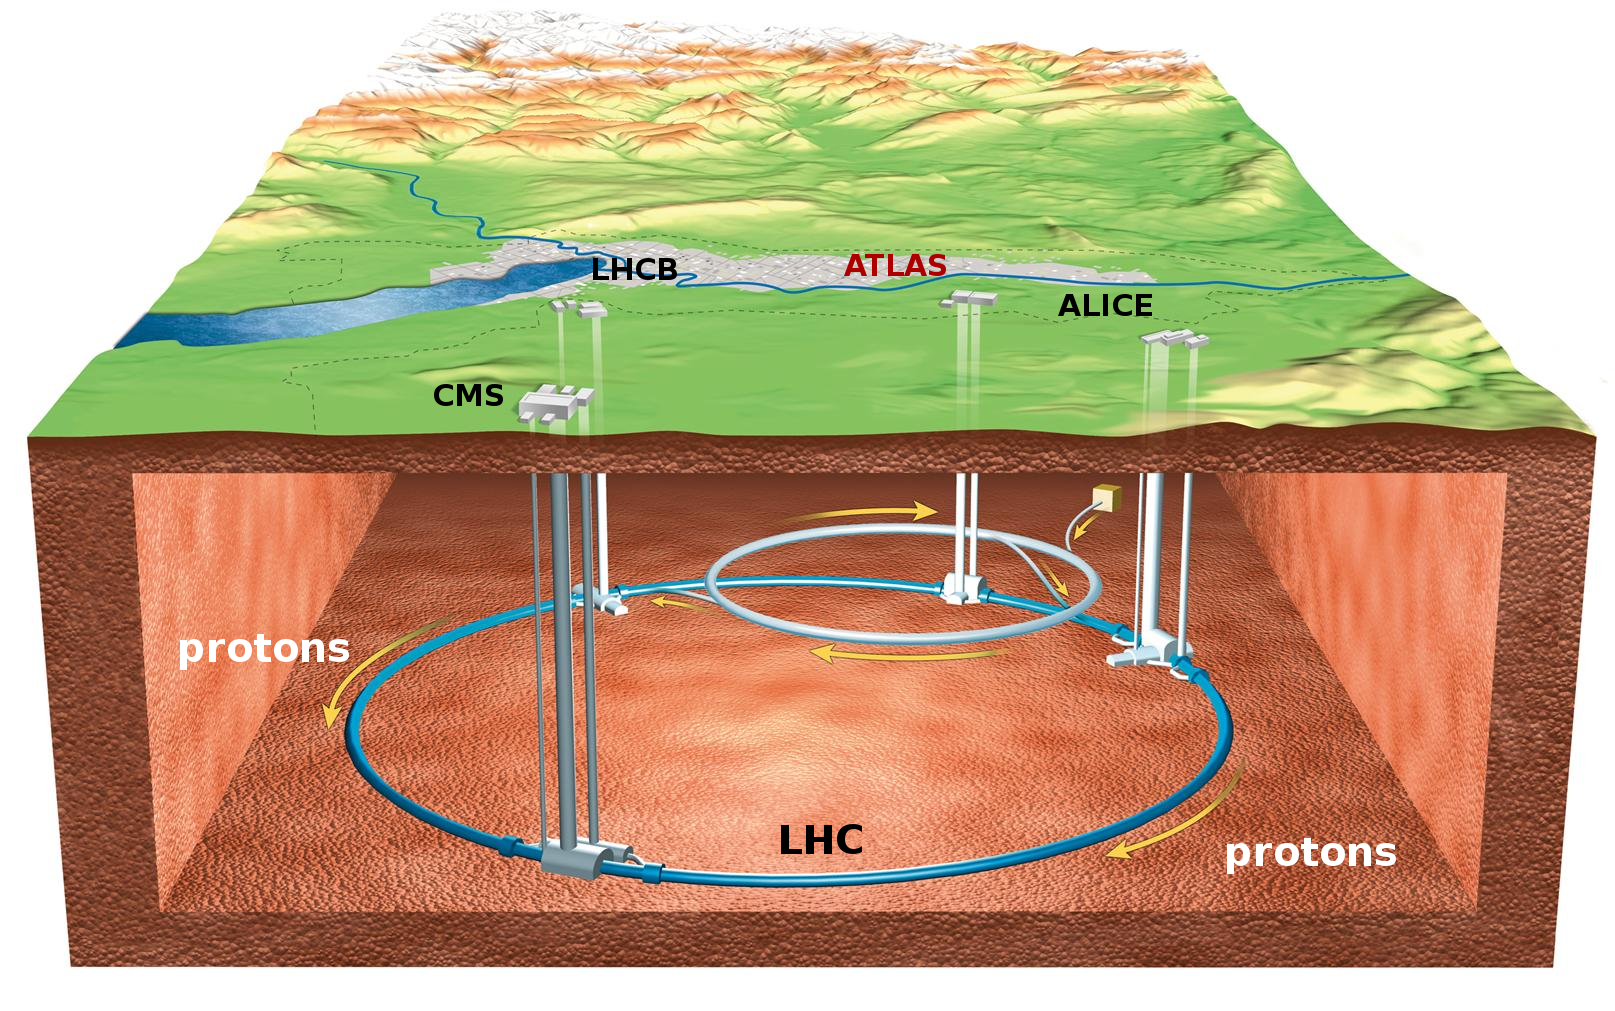
\includegraphics[width=.7\textwidth]{lhc-subterraneo}

\note<1>{
Qui dico che LHC è un sincrotrone che accelera protoni e li fa scontrare
in corrispondenza dei 4 esperimenti, tra i quali ATLAS che è quello di cui
ci siamo occupati. Poi compare l'itemize in cui dico che attualmente sono ad un'energia
di 13 TeV e che ci sono tot bunch ogni 25 ns
}

\onslide<2->{
\begin{itemize}
\item Durante la presa dati attuale (Run 2), i protoni collidono ad un'energia del centro di massa di 13 TeV
\item $\sim$ 2800 ``pacchetti'' (\textit{bunch}) di protoni collidono ogni 25 ns
\end{itemize}}

\end{frame}

%-----------------------------------------

\begin{frame}[t]
\frametitle{Tipi di collisione}
\note<1>{
Abbiamo visto che LHC accelera protoni e fa scontrare i bunch. Cosa succede in una singola
collisione? Pu\`o esserci collisione elastica, pu\`o esserci una collisione inelastica in cui si 
osservano un gran numero di prodotti finali, e ci sono
i processi hard, in cui i quark interagiscono direttamente per dare luogo a interazioni rare ``interessanti''.
}
Le collisioni possono essere:
\begin{itemize}
\item \textbf{elastiche}: i protoni rimangono intatti
\item \textbf{inelastiche}: lo stato finale è diverso da quello iniziale
	\setbeamercolor{local structure}{fg=red}
	\begin{itemize}
	\item \textbf{``hard''}: la collisione avviene direttamente tra partoni con produzione di uno stato finale raro ``interessante'' 
	\end{itemize}
\end{itemize}

\centering
\includegraphics[width=.7\textwidth]{protonCollision}


\end{frame}

%-----------------------------------------
\begin{frame}[t]
\frametitle{Numero di interazioni}

\note<1>{
Definisco R = L$\sigma$  e dico che il numero di interazioni per bunch è dato da N = L$\times \sigma_{inel.} \times 25$ ns
}

Il numero medio di interazioni per unit\`a di tempo \`e dato da\\
\medskip

\begin{columns}
\begin{column}{0.4\textwidth}
$$
\frac{dN}{dt} =\sigma \times \mathcal{L}
$$
\end{column}
\begin{column}{0.6\textwidth}
\end{column}
\end{columns}
\medskip
con:\\
\begin{itemize}
\item $\mathcal{L}$: luminosit\`a istantanea, termine geometrico che descrive la geometria del fascio 
\item $\sigma$: sezione d'urto del processo considerato
\end{itemize}

\bigskip 

\onslide<2->{
Il numero medio di interazioni per ``bunch-crossing'' \`e quindi:\\
\begin{columns}
\begin{column}{0.6\textwidth}
$$
\langle\mu\rangle = \sigma_{inel.} \times \mathcal{L} \times 25\ \mathrm{ns} \mathrm{\mathbf{\ \simeq 23\ }(Run 2)} 
$$
\end{column}
\begin{column}{0.4\textwidth}
\end{column}
\end{columns}

}
\end{frame}

%-----------------------------------------

\begin{frame}

\end{frame}

%-----------------------------------------

\end{document}